\subsection{Frequency, antenna and space correlation}
From \todo{ref to the place, where we talk about correlation and make the statement of the value}

\begin{minipage}{0.33\textwidth}
\begin{figure}[H]
% This file was created by matlab2tikz.
%
%The latest updates can be retrieved from
%  http://www.mathworks.com/matlabcentral/fileexchange/22022-matlab2tikz-matlab2tikz
%where you can also make suggestions and rate matlab2tikz.
%
\definecolor{mycolor1}{rgb}{0.00000,0.44700,0.74100}%
%
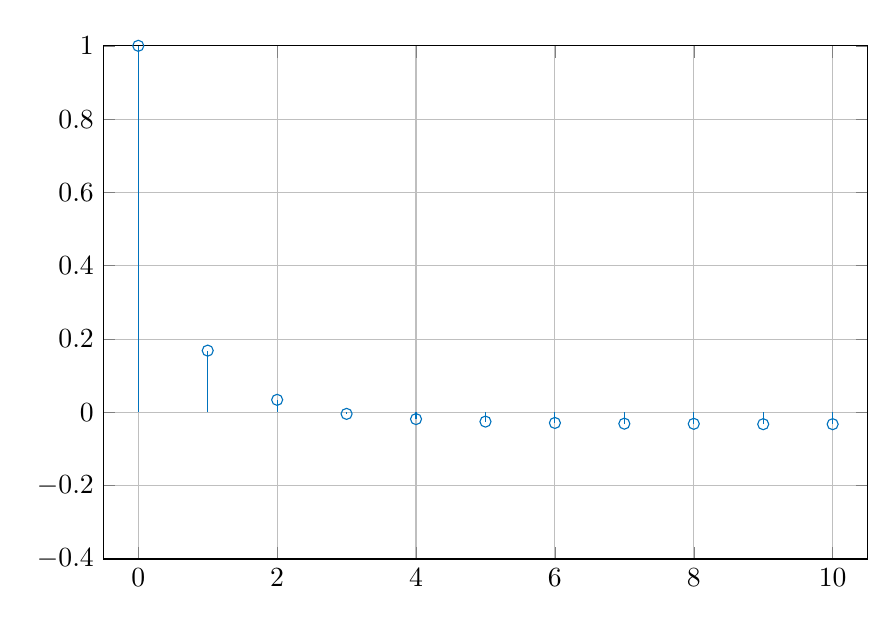
\begin{tikzpicture}

\begin{axis}[%
width=0.8\textwidth,
height=2.566in,
at={(0.758in,0.481in)},
scale only axis,
xmin=-0.5,
xmax=10.5,
ymin=-0.4,
ymax=1,
xmajorgrids,
ymajorgrids,
axis background/.style={fill=white}
]
\addplot[ycomb,color=mycolor1,solid,mark=o,mark options={solid},forget plot] plot table[row sep=crcr] {%
0	1\\
1	0.168482816521683\\
2	0.0342128083483619\\
3	-0.00408957803154558\\
4	-0.0183085697801844\\
5	-0.0251622968091291\\
6	-0.0288017885999447\\
7	-0.0307980799213752\\
8	-0.0311863299040153\\
9	-0.0322035626935004\\
10	-0.0321841811014383\\
};
\end{axis}
\end{tikzpicture}%
\caption{Hallos}
\label{1}
\end{figure}
\end{minipage}%
\begin{minipage}{0.33\textwidth}
\begin{figure}[H]
% This file was created by matlab2tikz.
%
%The latest updates can be retrieved from
%  http://www.mathworks.com/matlabcentral/fileexchange/22022-matlab2tikz-matlab2tikz
%where you can also make suggestions and rate matlab2tikz.
%
\definecolor{mycolor1}{rgb}{0.00000,0.44700,0.74100}%
%
\begin{tikzpicture}

\begin{axis}[%
width=0.8\textwidth,
height=0.7\textwidth,
at={(0.758in,0.481in)},
scale only axis,
xmin=-0.1,
xmax=2.1,
xtick={0, 1, 2},
xlabel={Lags},
xmajorgrids,
ymin=-0.4,
ymax=1,
%ylabel={Correlation},
ymajorgrids,
axis background/.style={fill=white},
legend style={legend cell align=left,align=left,draw=white!15!black}
]
\addplot[ycomb,color=mycolor1,solid,mark=o,mark options={solid}] plot table[row sep=crcr] {%
0	1\\
1	-0.309674488788906\\
2	-0.190325511211109\\
};
\addlegendentry{ACF};

\end{axis}
\end{tikzpicture}%
\caption{Hallos}
\label{2}
\end{figure}
\end{minipage}%
\begin{minipage}{0.33\textwidth}
\begin{figure}[H]
% This file was created by matlab2tikz.
%
%The latest updates can be retrieved from
%  http://www.mathworks.com/matlabcentral/fileexchange/22022-matlab2tikz-matlab2tikz
%where you can also make suggestions and rate matlab2tikz.
%
\definecolor{mycolor1}{rgb}{0.00000,0.44700,0.74100}%
%
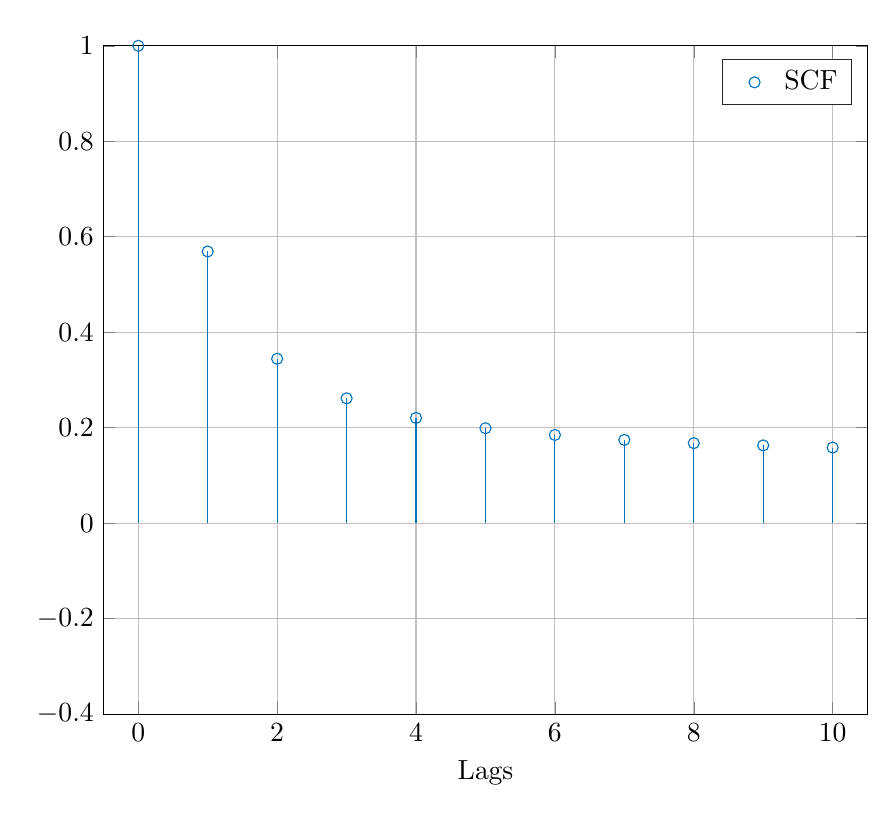
\begin{tikzpicture}

\begin{axis}[%
width=0.8\textwidth,
height=0.7\textwidth,
at={(0.756in,0.482in)},
scale only axis,
xmin=-0.5,
xmax=10.5,
xlabel={Lags},
xmajorgrids,
ymin=-0.4,
ymax=1,
%ylabel={Correlation},
ymajorgrids,
axis background/.style={fill=white},
legend style={legend cell align=left,align=left,draw=white!15!black}
]
\addplot[ycomb,color=mycolor1,solid,mark=o,mark options={solid}] plot table[row sep=crcr] {%
0	1\\
1	0.569162574789438\\
2	0.344435508447973\\
3	0.261498330064642\\
4	0.220468390451925\\
5	0.19896803835742\\
6	0.184853097999834\\
7	0.17444588999812\\
8	0.167644063920708\\
9	0.162911754175178\\
10	0.158398649695999\\
};
\addlegendentry{SCF};

\end{axis}
\end{tikzpicture}%
\caption{Hallos}
\label{3}
\end{figure}
\end{minipage}


\subsection{Approximate N Equivalent}


As seen in previous sections, the samples are correlated, both in frequency and space. As not all samples are independent, there is not enough independent samples to for filled the number of wanted independent samples, which was calculated in \autoref{sec:Brute}. To find the equivalent number of independent samples, that can be produces from the measurements, it will be looked at the how to lower the correlation between the samples. As seen from the previous sections, the big problem, is the correlation in space, which is the only place, where the correlation exceeds the maximum wanted correlation. From \todo{Ref to Rx in space}, it can be seen that the correlation between two adjacent samples is \todo{Number} in space. By removing every other sample, the correlation between adjacent samples will be removed and the correlation for one lag will nearly equal to the correlation for two lag, before removal of half the samples, seen in \todo{insert normal Rx and Rx2}.


The drawback from removal of half of the samples, is that the confidence level/interval wanted in \todo{ref to bruteforce part}, can not be for filled, as the number of independent samples is not high enough. With the lower number of independent samples, the wider the confidence interval or lower confidence level can be for filled. By cutting the sample pool down to half (2,092,230 samples), either the confidence level should be lowered to 76\% or the confidence interval widened to $\pm 1.33dB$ or both shall be lowered/widened. With the usage of the bootstrap method, the confidence level can be set at the wanted level and the confidence interval can then be found.


\subsection{CDF}
The CDF made from the measurements of the fading is shown in \autoref{CDFFinalBS}. Beside the CDF of the measurements, the 90\% confidence level interval is shown, made with the bootstrap method, which have run 100,000 times.

\begin{figure}[H]
% This file was created by matlab2tikz.
%
%The latest updates can be retrieved from
%  http://www.mathworks.com/matlabcentral/fileexchange/22022-matlab2tikz-matlab2tikz
%where you can also make suggestions and rate matlab2tikz.
%
\definecolor{mycolor1}{rgb}{0.00000,0.44700,0.74100}%
\definecolor{mycolor2}{rgb}{0.85000,0.32500,0.09800}%
\definecolor{mycolor3}{rgb}{0.92900,0.69400,0.12500}%
\definecolor{mycolor4}{rgb}{0.4940, 0.1840, 0.5560}%
%
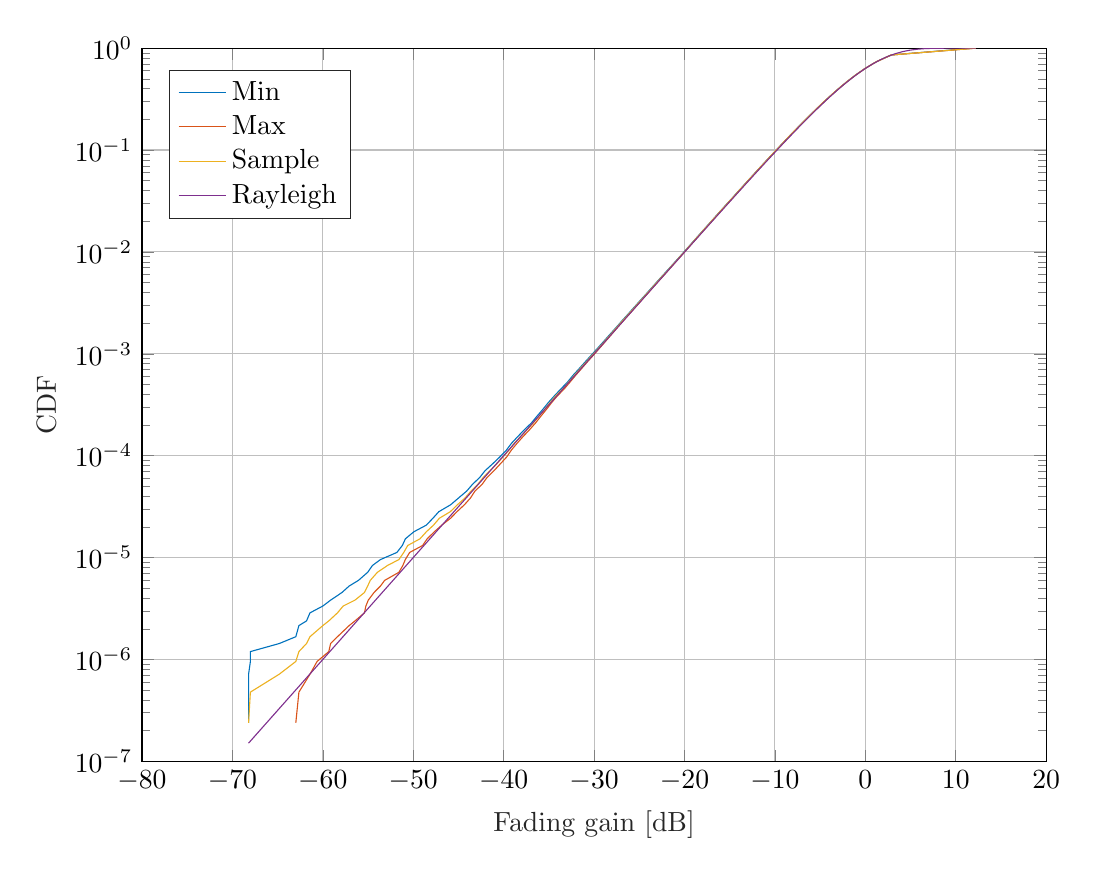
\begin{tikzpicture}

\begin{axis}[%
width=4.521in,
height=3.566in,
at={(0.758in,0.481in)},
scale only axis,
xmin=-80,
xmax=20,
xlabel style={font=\color{white!15!black}},
xlabel={Fading gain [dB]},
ymode=log,
ymin=1e-07,
ymax=1,
yminorticks=true,
ylabel style={font=\color{white!15!black}},
ylabel={CDF},
axis background/.style={fill=white},
xmajorgrids,
ymajorgrids,
legend style={at={(0.03,0.97)}, anchor=north west, legend cell align=left, align=left, draw=white!15!black}
]
\addplot [color=mycolor1]
  table[row sep=crcr]{%
-68.2110096592513	2.38979462105027e-07\\
-68.2110096592513	2.38979462105027e-07\\
-68.2110096592513	2.38979462105027e-07\\
-68.2110096592513	4.77958924210053e-07\\
-68.2110096592513	4.77958924210053e-07\\
-68.2110096592513	4.77958924210053e-07\\
-68.2110096592513	7.1693838631508e-07\\
-68.2110096592513	7.1693838631508e-07\\
-68.2110096592513	7.1693838631508e-07\\
-68.0097151399393	9.55917848420107e-07\\
-68.0097151399393	1.19489731052513e-06\\
-68.0097151399393	1.19489731052513e-06\\
-64.8166734306338	1.43387677263016e-06\\
-62.9863771783808	1.67285623473519e-06\\
-62.6440162806327	2.15081515894524e-06\\
-61.8030643971559	2.38979462105027e-06\\
-61.4203117587121	2.86775354526032e-06\\
-59.9985161369365	3.34571246947037e-06\\
-59.1355740602006	3.82367139368043e-06\\
-57.8863760614506	4.54060977999551e-06\\
-57.0865613837983	5.25754816631059e-06\\
-56.0604591827749	5.97448655262567e-06\\
-55.0373127063365	7.1693838631508e-06\\
-54.5129963452233	8.36428117367593e-06\\
-53.6260805121502	9.55917848420107e-06\\
-51.808335115529	1.12320347189363e-05\\
-51.2080103417404	1.31438704157765e-05\\
-50.8656140294929	1.52946855747217e-05\\
-49.9329752881246	1.7923459657877e-05\\
-48.5646784611454	2.07912132031373e-05\\
-47.8150369487296	2.43759051347127e-05\\
-47.1747472820195	2.81995765283932e-05\\
-45.8683353237914	3.29791657704937e-05\\
-44.9871986122314	3.84756933989093e-05\\
-44.0914311606797	4.4928138875745e-05\\
-43.4456160482323	5.23365022010008e-05\\
-42.6475646999491	6.11787422988868e-05\\
-42.0605846680829	7.12158797072979e-05\\
-41.2226743633778	8.31648528125493e-05\\
-40.4354193606139	9.70256616146408e-05\\
-39.7011242238561	0.000113276265037783\\
-39.147139735546	0.000131916663081975\\
-38.4457074477402	0.000153902773595637\\
-37.7167305259184	0.00017971255550298\\
-36.9321657726358	0.000209584988266108\\
-36.3133129747694	0.000244475989733442\\
-35.6652847986588	0.000285102498291297\\
-35.0526311091789	0.000332659411250197\\
-34.3760634514811	0.000388102646458563\\
-33.6627095375474	0.000452627101226921\\
-32.9383151044303	0.000527905631790004\\
-32.3251969323066	0.000615850073844654\\
-31.6323951726943	0.00071837226308771\\
-30.9594714391043	0.000838100973602329\\
-30.2697757571462	0.000977664979471664\\
-29.5898359988414	0.00114040999316519\\
-28.9152019894879	0.00133015968607658\\
-28.2476390646933	0.00155169364744794\\
-27.5690927911693	0.00181003044598347\\
-26.9096611998945	0.00211138354769791\\
-26.2222216444869	0.00246316131591651\\
-25.5527192546351	0.00287325007288874\\
-24.8783691997257	0.00335144797656089\\
-24.1969945680687	0.00390970400003824\\
-23.5249012466879	0.00456044507535022\\
-22.8506178328178	0.00531992180592\\
-22.1645657934235	0.00620557969248123\\
-21.4814600973437	0.00723892688662336\\
-20.7990062560447	0.00844410031401901\\
-20.1227479111593	0.00985025546904499\\
-19.4533750883144	0.0114901325380097\\
-18.7879510183893	0.0134034021116225\\
-18.11737882869	0.0156349923287593\\
-17.4439705115225	0.0182381956094693\\
-16.7687607321705	0.0212749076344379\\
-16.0925979696037	0.0248173002012207\\
-15.4145418534632	0.0289494940804787\\
-14.725921602577	0.033769470851675\\
-14.0476022031757	0.0393921796360821\\
-13.3635807512048	0.0459509709735545\\
-12.6768389867612	0.053601898452847\\
-11.9881607500358	0.0625268254446213\\
-11.2966277760374	0.0729374877523026\\
-10.5940040241995	0.0850817070780937\\
-9.88832382352862	0.0992479316327555\\
-9.17878765657663	0.115772883478394\\
-8.46481660429262	0.135049205871247\\
-7.73834288203237	0.157535022440171\\
-6.99807258551004	0.183764691262433\\
-6.24631661723323	0.214361948734126\\
-5.4759007806751	0.250053292420049\\
-4.68523948296265	0.291687577369601\\
-3.86815019946715	0.340253939576433\\
-3.01508243691754	0.396906888821975\\
-2.11164808069142	0.462992357436802\\
-1.13797902811865	0.540081157425331\\
-0.0595261498871336	0.630005305344059\\
1.19898648150126	0.734902233502053\\
2.86256679049623	0.857264258709607\\
11.9680456293704	1\\
};
\addlegendentry{Min}

\addplot [color=mycolor2]
  table[row sep=crcr]{%
-62.9863771783808	2.38979462105027e-07\\
-62.9863771783808	2.38979462105027e-07\\
-62.9863771783808	2.38979462105027e-07\\
-62.6440162806327	4.77958924210053e-07\\
-62.6440162806327	4.77958924210053e-07\\
-62.6440162806327	4.77958924210053e-07\\
-61.4203117587121	7.1693838631508e-07\\
-61.4203117587121	7.1693838631508e-07\\
-61.4203117587121	7.1693838631508e-07\\
-60.6336777269018	9.55917848420107e-07\\
-59.3401343530983	1.19489731052513e-06\\
-59.3401343530983	1.19489731052513e-06\\
-59.1355740602006	1.43387677263016e-06\\
-58.3785063400625	1.67285623473519e-06\\
-57.0865613837983	2.15081515894524e-06\\
-56.444106415324	2.38979462105027e-06\\
-55.3967704494347	2.86775354526032e-06\\
-55.2381930601198	3.34571246947037e-06\\
-54.9727246723381	3.82367139368043e-06\\
-54.3383407041317	4.54060977999551e-06\\
-53.6260805121502	5.25754816631059e-06\\
-53.1631074106005	5.97448655262567e-06\\
-51.5860452686304	7.1693838631508e-06\\
-51.1500489743732	8.36428117367593e-06\\
-50.8775668224382	9.55917848420107e-06\\
-50.3952036874581	1.12320347189363e-05\\
-48.9661937487716	1.31438704157765e-05\\
-48.4579701962169	1.52946855747217e-05\\
-47.6704936771493	1.7923459657877e-05\\
-46.8511092276623	2.07912132031373e-05\\
-45.8645645025135	2.43759051347127e-05\\
-45.166065931658	2.81995765283932e-05\\
-44.3450506560681	3.29791657704937e-05\\
-43.6678872485078	3.84756933989093e-05\\
-43.1791524561151	4.4928138875745e-05\\
-42.3851248085774	5.23365022010008e-05\\
-41.8337173894218	6.11787422988868e-05\\
-41.0711744934229	7.12158797072979e-05\\
-40.3678651666811	8.31648528125493e-05\\
-39.6686728490359	9.70256616146408e-05\\
-39.1527262775304	0.000113276265037783\\
-38.5321372890392	0.000131916663081975\\
-37.8631393924066	0.000153902773595637\\
-37.140589389943	0.00017971255550298\\
-36.4762679448601	0.000209584988266108\\
-35.8803897583857	0.000244475989733442\\
-35.2654230564002	0.000285102498291297\\
-34.6854390450426	0.000332659411250197\\
-34.0399464712618	0.000388102646458563\\
-33.2979444688087	0.000452627101226921\\
-32.6612779841195	0.000527905631790004\\
-32.0315470964707	0.000615850073844654\\
-31.3745387536688	0.00071837226308771\\
-30.7193423898906	0.000838100973602329\\
-30.0364045496681	0.000977664979471664\\
-29.3767040268811	0.00114040999316519\\
-28.7202288623912	0.00133015968607658\\
-28.0675465918805	0.00155169364744794\\
-27.4196791031216	0.00181003044598347\\
-26.7635602371125	0.00211138354769791\\
-26.0843214959411	0.00246316131591651\\
-25.4221763271499	0.00287325007288874\\
-24.7549437322726	0.00335144797656089\\
-24.0821180037386	0.00390970400003824\\
-23.4184194677437	0.00456044507535022\\
-22.7507526131484	0.00531992180592\\
-22.0643678661751	0.00620557969248123\\
-21.3954528690652	0.00723892688662336\\
-20.7277835285591	0.00844410031401901\\
-20.0515086533784	0.00985025546904499\\
-19.3902406579038	0.0114901325380097\\
-18.7278248792547	0.0134034021116225\\
-18.0626484177151	0.0156349923287593\\
-17.3919345527781	0.0182381956094693\\
-16.7203270784246	0.0212749076344379\\
-16.0473716177478	0.0248173002012207\\
-15.3717167183636	0.0289494940804787\\
-14.6882080507172	0.033769470851675\\
-14.0121789823898	0.0393921796360821\\
-13.3298515329136	0.0459509709735545\\
-12.6474455107362	0.053601898452847\\
-11.9587133864622	0.0625268254446213\\
-11.2696796711578	0.0729374877523026\\
-10.5696398943488	0.0850817070780937\\
-9.86542344409112	0.0992479316327555\\
-9.1579227575183	0.115772883478394\\
-8.4451223163299	0.135049205871247\\
-7.72097944756374	0.157535022440171\\
-6.98163565797006	0.183764691262433\\
-6.23091515138027	0.214361948734126\\
-5.46228056495459	0.250053292420049\\
-4.67227435513875	0.291687577369601\\
-3.85610450789956	0.340253939576433\\
-3.00359708496823	0.396906888821975\\
-2.10113619390274	0.462992357436802\\
-1.12791338599333	0.540081157425331\\
-0.0502216274060202	0.630005305344059\\
1.20797074210325	0.734902233502053\\
2.87148875177718	0.857264258709607\\
12.2257224522847	1\\
};
\addlegendentry{Max}

\addplot [color=mycolor3]
  table[row sep=crcr]{%
-68.2110096592513	2.38979462105027e-07\\
-68.2110096592513	2.38979462105027e-07\\
-68.2110096592513	2.38979462105027e-07\\
-68.0097151399393	4.77958924210053e-07\\
-68.0097151399393	4.77958924210053e-07\\
-68.0097151399393	4.77958924210053e-07\\
-64.8166734306338	7.1693838631508e-07\\
-64.8166734306338	7.1693838631508e-07\\
-64.8166734306338	7.1693838631508e-07\\
-62.9863771783808	9.55917848420107e-07\\
-62.6440162806327	1.19489731052513e-06\\
-62.6440162806327	1.19489731052513e-06\\
-61.8030643971559	1.43387677263016e-06\\
-61.4203117587121	1.67285623473519e-06\\
-59.9985161369365	2.15081515894524e-06\\
-59.3401343530983	2.38979462105027e-06\\
-58.3785063400625	2.86775354526032e-06\\
-57.7481209120663	3.34571246947037e-06\\
-56.444106415324	3.82367139368043e-06\\
-55.3967704494347	4.54060977999551e-06\\
-55.0373127063365	5.25754816631059e-06\\
-54.7524652239827	5.97448655262567e-06\\
-53.9636508575883	7.1693838631508e-06\\
-52.8477396996391	8.36428117367593e-06\\
-51.5860452686304	9.55917848420107e-06\\
-51.0494172432138	1.12320347189363e-05\\
-50.6103550594968	1.31438704157765e-05\\
-49.250974367012	1.52946855747217e-05\\
-48.5481633258799	1.7923459657877e-05\\
-47.7679593085902	2.07912132031373e-05\\
-47.0996659103971	2.43759051347127e-05\\
-45.9025330713494	2.81995765283932e-05\\
-45.1210769481119	3.29791657704937e-05\\
-44.2704326549902	3.84756933989093e-05\\
-43.6192459081114	4.4928138875745e-05\\
-42.8666360745012	5.23365022010008e-05\\
-42.2566046404878	6.11787422988868e-05\\
-41.5193936351877	7.12158797072979e-05\\
-40.770890357656	8.31648528125493e-05\\
-40.0821084592503	9.70256616146408e-05\\
-39.4187232573994	0.000113276265037783\\
-38.8554059458105	0.000131916663081975\\
-38.1289750187655	0.000153902773595637\\
-37.4145651196132	0.00017971255550298\\
-36.7212978502416	0.000209584988266108\\
-36.0826678316439	0.000244475989733442\\
-35.4686472524818	0.000285102498291297\\
-34.8582416427754	0.000332659411250197\\
-34.2096345341231	0.000388102646458563\\
-33.4501488589808	0.000452627101226921\\
-32.8136808619326	0.000527905631790004\\
-32.163145835631	0.000615850073844654\\
-31.5159363723506	0.00071837226308771\\
-30.833128222479	0.000838100973602329\\
-30.1686401472903	0.000977664979471664\\
-29.4850461489385	0.00114040999316519\\
-28.8213408716825	0.00133015968607658\\
-28.1597602635248	0.00155169364744794\\
-27.498343553035	0.00181003044598347\\
-26.8406337645007	0.00211138354769791\\
-26.1546662653618	0.00246316131591651\\
-25.4856173328105	0.00287325007288874\\
-24.8162453705439	0.00335144797656089\\
-24.1417693615402	0.00390970400003824\\
-23.4721417638783	0.00456044507535022\\
-22.8046021225034	0.00531992180592\\
-22.1089359169015	0.00620557969248123\\
-21.4396485718651	0.00723892688662336\\
-20.7648772213262	0.00844410031401901\\
-20.086569269905	0.00985025546904499\\
-19.422428768153	0.0114901325380097\\
-18.7599926207705	0.0134034021116225\\
-18.0904229133163	0.0156349923287593\\
-17.4178537656637	0.0182381956094693\\
-16.7455555809535	0.0212749076344379\\
-16.0702080584915	0.0248173002012207\\
-15.3922605055207	0.0289494940804787\\
-14.706733272626	0.033769470851675\\
-14.0305222056965	0.0393921796360821\\
-13.3463206244526	0.0459509709735545\\
-12.6618161043484	0.053601898452847\\
-11.9741383511965	0.0625268254446213\\
-11.2833412072204	0.0729374877523026\\
-10.5816982084268	0.0850817070780937\\
-9.87645579084854	0.0992479316327555\\
-9.16830342925416	0.115772883478394\\
-8.45467008880847	0.135049205871247\\
-7.72959925946455	0.157535022440171\\
-6.98960709738607	0.183764691262433\\
-6.23862292036003	0.214361948734126\\
-5.46877497627373	0.250053292420049\\
-4.67861574208366	0.291687577369601\\
-3.86199489621806	0.340253939576433\\
-3.00932724828141	0.396906888821975\\
-2.10635361124778	0.462992357436802\\
-1.13307303936403	0.540081157425331\\
-0.0548778964736532	0.630005305344059\\
1.20345603455642	0.734902233502053\\
2.86714851530094	0.857264258709607\\
12.2257224522847	1\\
};
\addlegendentry{Sample}

\addplot [color=mycolor4,solid]
  table[row sep=crcr]{%
-68.2110096592513	1.50972901402646e-07\\
-68.2110096592513	1.50972901402646e-07\\
-68.2110096592513	1.50972901402646e-07\\
-68.2110096592513	1.50972901402646e-07\\
-64.8166734306338	3.29862225978417e-07\\
-64.8166734306338	3.29862225978417e-07\\
-64.8166734306338	3.29862225978417e-07\\
-62.9863771783808	5.02761684839648e-07\\
-62.6440162806327	5.43999190916189e-07\\
-61.4203117587121	7.21055456343045e-07\\
-60.6336777269018	8.64235376374367e-07\\
-59.3401343530983	1.16408933903411e-06\\
-58.3785063400625	1.45261007011843e-06\\
-57.8863760614506	1.62690442573332e-06\\
-57.0865613837983	1.9558855444135e-06\\
-56.2640834688009	2.36369338535436e-06\\
-55.3967704494347	2.88617279242676e-06\\
-54.5129963452233	3.53752564818954e-06\\
-53.6260805121502	4.33901355223476e-06\\
-52.8477396996391	5.19068773274789e-06\\
-51.808335115529	6.59424466298297e-06\\
-51.2335225394739	7.52741935661216e-06\\
-50.3952036874581	9.13014445014237e-06\\
-49.250974367012	1.18822854989764e-05\\
-48.7531821751098	1.33253581002801e-05\\
-47.9342988082392	1.60903920185529e-05\\
-47.0996659103971	1.94997558889964e-05\\
-46.2180867037292	2.38883493837161e-05\\
-45.4693715783321	2.83828942324593e-05\\
-44.6184038894186	3.45264648679011e-05\\
-43.8007947762002	4.1678441598858e-05\\
-43.0069103086247	5.00377880663372e-05\\
-42.2054341314618	6.01787993705916e-05\\
-41.375348198628	7.28533220063499e-05\\
-40.5873845302451	8.73459111149222e-05\\
-39.7704856340632	0.000105421342778689\\
-38.9565011745757	0.000127151729109931\\
-38.1498623564989	0.000153101877521711\\
-37.3227091045878	0.000185220420714005\\
-36.5236581392873	0.000222631102938853\\
-35.7133189395457	0.000268293308071432\\
-34.9007422681537	0.000323486022222652\\
-34.0865647668023	0.000390174411719957\\
-33.2748499401011	0.000470341015727627\\
-32.4622924000808	0.000567084255998607\\
-31.6467384948507	0.000684191284853641\\
-30.8362609494202	0.000824507867212221\\
-30.0241732106052	0.000993955073611663\\
-29.209597003383	0.00119889136875362\\
-28.3986444198802	0.00144484621506336\\
-27.5858413365337	0.00174195659948351\\
-26.7740081825629	0.00209963040602013\\
-25.9616419310967	0.00253096206009951\\
-25.1482790923368	0.00305146665936729\\
-24.3358399410187	0.00367803708299952\\
-23.5240456664277	0.00443232078902567\\
-22.7114945184127	0.00534180462696821\\
-21.8987538460546	0.00643758457158361\\
-21.0863209149848	0.00775671954162982\\
-20.2739299412833	0.00934479682612888\\
-19.4615124357845	0.0112562299168664\\
-18.6489708222903	0.0135563393562459\\
-17.8364997462625	0.0163222993822064\\
-17.0240289201783	0.0196469654492744\\
-16.2115226805754	0.0236408393834987\\
-15.3990261778159	0.0284346862688158\\
-14.5865067520205	0.0341836545859274\\
-13.7740424091047	0.0410696605247216\\
-12.9615421494463	0.049307400496136\\
-12.1490297705241	0.0591460028156858\\
-11.3365516149888	0.0708728963741718\\
-10.5240625928983	0.0848182973600722\\
-9.71157214658825	0.101354631038396\\
-8.89906767190964	0.120896476296817\\
-8.08657847793165	0.143893976773573\\
-7.27406899262304	0.170824844646777\\
-6.46159752980708	0.202170593043456\\
-5.64910699945253	0.23839415508501\\
-4.83661628132355	0.279889798910119\\
-4.02412151827199	0.326927439723138\\
-3.21162375382428	0.379575133378583\\
-2.39913629691027	0.437607002309584\\
-1.58664596098345	0.500407015396857\\
-0.774152736194334	0.566874960139745\\
0.0383458269129778	0.63536869074599\\
0.850836897357556	0.70371112917412\\
1.66332467266342	0.769307632272229\\
2.47582816982846	0.829395865496377\\
3.28831017181545	0.881425652791366\\
4.10080734238841	0.923531291207476\\
4.91329501422534	0.954940444949963\\
5.72578667828212	0.976185918103421\\
6.53834362515757	0.988962403648043\\
7.35083903054455	0.995632449454543\\
8.16344081637964	0.998572099834011\\
8.97581652258484	0.999628949908912\\
9.78853581621829	0.999926978009124\\
10.6040834657513	0.999989791979648\\
11.4226799871078	0.999999058807792\\
12.2257224522847	0.999999943805951\\
};
\addlegendentry{Rayleigh}
\end{axis}
\end{tikzpicture}%

\caption{CDF of the measurements of the fading channel. The min and max is the 90\% confidence level made with the bootstrap method, run 100,000 times.}
\label{CDFFinalBS}
\end{figure}

From the bootstrap, the confidence interval can be found for the $10^{-5}$ point, which is [-53.59; -51.13]. The interval is bigger than the interval, which was calculated in \autoref{sec:Brute}. But with a lower number of independent samples, shown in previous section, this is expected.


\section{Results}